\documentclass[12pt,a4paper]{article}
\usepackage[left=2.00cm, right=2.00cm, top=2.00cm, bottom=2.00cm]{geometry}
\usepackage[tiny]{titlesec}
\usepackage[utf8x]{inputenc}
\usepackage[polish]{babel}
\usepackage[T1]{fontenc}
\usepackage{ucs}
\usepackage{amsmath}
\usepackage{amsfonts}
\usepackage{graphicx}
\usepackage{multicol}
\usepackage{hyperref}


\hypersetup{
	colorlinks   = true,    % Colours links instead of ugly boxes
	urlcolor     = blue,    % Colour for external hyperlinks
	linkcolor    = blue,    % Colour of internal links
	citecolor    = red      % Colour of citations
}

\title{Pytania i odpowiedzi na obronę pracy inżynierskiej}
\author{
	Zachodniopomorski Uniwersytet Technologiczny\\
	Wydział Informatyki\\
	Szczecin
}
\date{\today}

\begin{document}
	\maketitle

	\section{Co to jest algorytm - cechy i właściwości}
	Algorytm jest skończonym, uporządkowanym ciągiem jasno zdefiniowanych czynności, koniecznych do wykonania postawionego  zadania.
	Cechy algorytmów:
	\begin{itemize}
		\item \textbf{poprawność} - algorytm daje oczekiwane wyniki,
		\item \textbf{jednoznaczność} - zawsze daje te same wyniki przy takich samych danych wejściowych,
		\item \textbf{skończoność} - wykonuje się w skończonej liczbie kroków,
		\item \textbf{sprawność} - czasowa - szybkość działania i pamięciowa.
	\end{itemize}
	Właściwości algorytmów:
	\begin{itemize}
		\item \textbf{efektywność} - algorytm powinien osiągać efekt końcowy możliwie niskim kosztem,
		\item \textbf{zgodność ze specyfikacją},
		\item \textbf{właściwość stopu} - algorytm powinien zatrzymać się w skończonym czasie (po wykonaniu lub mimo niewykonania postawionego zadania).
	\end{itemize}

	\section{Porównać pojęcia program, algorytm, procedura, funkcja, agent programowy.}
	\begin{itemize}
		\item \textbf{Program} - zaimplementowany algorytm w sposób zrozumiały dla komputera/maszyny go wykonującej.
		\item\textbf{ Procedura} - program w trakcie wykonania. Wykonuje operacje, ale nie zwraca wartości.
		\item \textbf{Funkcja} - część składowa programu zwracająca wartość
		\item \textbf{Agent programowy (zwany także systemem agentowym, agentem)} - system oparty na wiedzy. Definiuje się go jako autonomiczny program umieszczony w określonym otoczeniu (i będący jego częścią), który potrafi analizować to otoczenie i oddziaływać na nie w czasie, dążyć do wyznaczonych celów i symulować wpływ zmian tego otoczenia.
	\end{itemize}

	\section{Rodzaje zabezpieczeń systemów komputerowych}
	\begin{itemize}
		\item \textbf{fizyczne} - wszelkie zabezpieczenia przed otwarciem pokrywy komputera, zamki, blokady, zabezpieczenia antykradzieżowe, kontrola dostępu do obiektów i pomieszczeń, systemy przeciwpożarowe,
		\item \textbf{techniczne} - software, oprogramowanie antywirusowe, kontrola dostępu, szyfrowanie informacji
		\item \textbf{organizacyjne} - regulaminy dla osób korzystających z systemów informatycznych, polityka bezpieczeństwa,
		\item \textbf{personalne} - sprawdzanie pracowników dopuszczonych do danych o szczególnym znaczeniu, przestrzeganie odpowiednich procedur zwalniania i zatrudniania pracowników, szkolenia.
	\end{itemize}

	\section{Urządzenia wejścia i wyjścia}
	Urządzenia służące do wydobywania/przekazywania informacji z/do komputera, na przykład: mysz komputerowa, klawiatura, monitor, drukarka, skaner.

	\section{Scharakteryzować architekturę klient-serwer oraz klient-broker-serwer.}
	\begin{itemize}
		\item  \textbf{Klient-serwer} - program klienta (aktywny) wysyła żądania do serwera, który te zapytania przetwarza i dostarcza odpowiednią usługę. Z reguły serwer (pasywny) jest jeden i może obsługiwać wiele klientów.
		\item \textbf{Klient-broker-serwer} - pomiędzy klientem a serwerem jest pośrednik (broker), który jest odpowiedzialny za odbieranie wszystkich wiadomości, ich filtrowanie, określanie kto jest odbiorcą wiadomości oraz ich przesyłanie. Odpowiada również za przechowywanie danych o sesjach oraz autoryzację klientów.
	\end{itemize}

	\section{Wymienić i omówić metody wdrażania systemów informatycznych.}
	Odpowiedź

	\section{Scharakteryzować podstawowe modele baz danych.}
	\begin{itemize}
		\item  \textbf{Hierarchiczny} - w tym modelu przechowywane dane są zorganizowane w postaci drzewa. Informacja jest zawarta w dokumentach oraz w strukturze drzewa (podobnej do drzewa folderów na dysku komputera).
		\item  \textbf{Sieciowy} - uogólniony model hierarchiczny, rekordy mogą przyjmować strukturę dowolnego grafu.
		\item  \textbf{Relacyjny} - rekordy są grupowane w relacje (tabele). Dla każdej relacji musi zostać wybrany klucz główny, jednoznacznie identyfikujący dany rekord. Klucz obcy pozwala na powiązanie relacji między sobą (skrót myślowy). Większość relacyjnych baz danych korzysta z języka zapytań SQL. W modelu relacyjnym abstrahujemy od kolejności wierszy (rekordów) i kolumn (pól w rekordzie). Wiersz reprezentuje jeden rekord informacji np. osobę. Liczba kolumn jest z góry ustalona. Z każdą kolumną jest związana jej nazwa oraz dziedzina, określająca zbiór wartości, jakie mogą wystąpić w kolumnie.
		\item  \textbf{Obiektowy} - dane przyjmują postać obiektów. W przeciwieństwie do modelu relacyjnego, rekordy i relacje między nimi przechowywane są bezpośrednio (w formie obiektów, czyli struktur zwanych klasami), bez podziału na wiersze i kolumny.
	\end{itemize}

	\section{Czym wyróżnia się rozproszonych system informatycznych od innych.}
	W rozproszonych systemach informatycznych obliczenia wykonywane są na wielu komputerach, w potencjalnie różnych lokalizacjach.

	\section{Porównaj metody analizy obiektowej i strukturalnej w projektowaniu systemów informatycznych.}
	\begin{itemize}
		\item W podejściu \textbf{strukturalnym} dąży się do formalnej analizy systemu. W wyniku tej analizy tworzone są hierarchiczne struktury, których elementami są procesy, dane i związki zachodzące między nimi. Cechą charakterystyczną tego podejścia jest oddzielne modelowanie danych i procesów, wykorzystujące diagramowe i macierzowe metody i techniki.
		\item Podstawową różnicą między podejściem strukturalnym a \textbf{obiektowym} jest zintegrowane, jednoczesne modelowanie danych i procesów dziedziny przedmiotowej. System w podejściu obiektowym stanowi kolekcję różnych rodzajów, wzajemnie powiązanych elementów zwanych obiektami, spełniających w nim określoną rolę. Pojęcia klasy i obiektu umożliwiły powiązanie atrybutów (danych) i operacji (usług) w elementy, które łatwo przenieść koncepcyjnie na obiekty świata rzeczywistego.
	\end{itemize}

	\section{Scharakteryzować standardowy język zapytań do baz danych.}
	Odpowiedź

	\section{Na czym polega polimorfizm metod w programowaniu obiektowym i po co się go stosuje?}
	Polega na przedefiniowaniu metod klasy nadrzędnej w klasie pochodnej. Polimorfizm pozwala traktować różnorodne dane w ten sam sposób. Przykładowo mamy wiele klas (dziedziczących z jednej klasy abstrakcyjnej) dla różnych rodzajów figur geometrycznych a dla każdej z tych figur możemy policzyć jej pole. Polimorfizm pozwala nam w każdej z tych klas zaimplementować metodę wirtualną o takiej samej nazwie np. ObliczPole() i w zależności od typu obiektu w momencie wywołania metody zostanie wykonana ta prawidłowa. Pozwala to na odseparowanie implementacji od interfejsu, co z kolei ułatwia rozszerzanie funkcjonalności.

	\section{Wymienić i scharakteryzować metody testowania oprogramowania.}
	Ze względu na poziom szczegółowości:
		\begin{itemize}
			\item Testy jednostkowe: testowaniu podlegają najmniejsze elementy programu (np. pojedyncze funkcje).
			\item Testy integracyjne: testowaniu podlega komunikacja między komponentami systemu, w celu sprawdzenia poprawności interakcji między nimi.
			\item Testy systemowe: testowaniu podlega cały zintegrowany system w celu sprawdzenia, czy spełnia postawione mu wymagania.
			\item Testy akceptacyjne: sprawdzana jest gotowość systemu do wypuszczenia na rynek.
		\end{itemize}
	Ze względu na szczegóły implementacyjne:
		\begin{itemize}
			\item Testy funkcjonalne (czarnej skrzynki): implementacja nie jest znana, testowana jest funkcjonalność i warstwa interfejsu systemu.
			\item Testy strukturalne (białej skrzynki): implementacja jest znana, testowane są ścieżki przepływu sterowania (np. warunki).
		\end{itemize}


	\section{Wymienić metody ochrony danych w systemach baz danych.}
	\begin{multicols}{2}
		\begin{itemize}
			\item Kontrola dostępu,
			\item audyt wykonywanych operacji,
			\item uwierzytelnianie,
			\item szyfrowanie danych,
			\item kontrola integralności danych,
			\item kopie zapasowe,
			\item replikacja danych,
			\item mechanizm transakcji,
			\item ochrona w warstwie aplikacji.
		\end{itemize}
	\end{multicols}

	\section{Rola sterowników w dostępie do baz danych.}
	Sterowniki dla baz danych to programy implementujące protokół pozwalający na połączenie z bazą danych. Łączy interfejs użytkownika z konkretną bazą danych (np. JDBC, MySQL). Sterownik tłumaczy zapytania zadane przez użytkownika na język zrozumiały dla danego DBMS. Pozwala to na ujednolicenie interfejsu programistycznego komunikacji z systemami bazodanowymi.

	\section{Zarządzanie procesami w systemach operacyjnych.}
	Procesami zarządza planista (scheduler), który jest odpowiedzialny za rozpoczynanie, wznawianie i kończenie procesów oraz przełączanie kontekstu pomiędzy procesami. System operacyjny dostarcza mechanizmy umożliwiające komunikację między procesami oraz synchronizację. Planowanie procesów polega na wskazywaniu procesu, któremu ma być w danej chwili przydzielony procesor. W szczególności oznacza to decydowanie, kiedy i który proces ma przejść ze stanu gotowy do stanu aktywny. W systemie w każdej chwili może być aktywnych co najwyżej tyle procesów ile jest procesorów. W każdej chwili proces jest w jakimś stanie. Ten stan zmienia się w miarę postępu wykonania procesu. Oto możliwe stany:
	
	\begin{itemize}
		\item \textbf{Nowy} (proces właśnie utworzono) - może przejść jedynie do stanu gotowy. Dzieje się tak, gdy system załaduje program do pamięci.
		\item \textbf{Aktywny} (proces jest właśnie wykonywany przez procesor) - może przejść do jednego z trzech stanów:
		\begin{itemize}
			\item gotowy - gdy planista odbierze procesowi procesor,
			\item czekający - gdy proces rozpocznie oczekiwanie na jakieś zdarzenie, np. zleci operację wejścia-wyjścia i czeka na jej wykonanie,
			\item zakończony - gdy proces zakończy działanie.
		\end{itemize}
		\item \textbf{Czekający} - proces czeka na zajście jakiegoś zdarzenia (np. wykonanie operacji wejścia-wyjścia) -  może przejść jedynie do stanu gotowy. Dzieje się tak, gdy nastąpi oczekiwane przezeń zdarzenie, np. ukończenie operacji wejścia-wyjścia.
		\item \textbf{Gotowy} (proces czeka na przydzielenie mu procesora) - może przejść jedynie do stanu aktywny. Dzieje się tak, gdy moduł systemu operacyjnego zwany planistą przydzieli temu procesowi procesor.
		\item \textbf{Zakończony} (proces zakończył działanie) - nie może już zmienić swojego stanu.
	\end{itemize}

	\section{Co to jest system komputerowy, informacyjny, informatyczny.}
	\begin{itemize}	
		\item System komputerowy: sprzęt i oprogramowanie do przetwarzania danych. 
		\item System informacyjny: system, który przetwarza dane w informacje, gromadzi je i przesyła. 
		\item System informatyczny: część systemu informacyjnego, wykorzystująca system komputerowy.
	\end{itemize}


	\section{Powody tworzenia systemów rozproszonych.}
	\begin{itemize}
		\item \textbf{Dzielenie zasobów} (ang. resource sharing) – wielu użytkowników systemu może korzystać z danego zasobu (np. drukarek, plików, usług, itp.).
		
		\item \textbf{Otwartość} (ang. openness) – podatność na rozszerzenia, możliwość rozbudowy systemu zarówno pod względem sprzętowym, jak i oprogramowania.
		
		\item \textbf{Współbieżność} (ang. concurrency) – zdolność do przetwarzania wielu zadań jednocześnie.
		
		\item \textbf{Skalowalność} (ang. scalability) – cecha systemu umożliwiająca zachowanie podobnej wydajności systemu przy zwiększaniu skali systemu (np. liczby procesów, komputerów, itp.).
		
		\item \textbf{Tolerowanie awarii} (ang. fault tolerance) – właściwość systemu umożliwiająca działania systemu mimo pojawiania się błędów i (lub) uszkodzeń (np. przez utrzymywanie nadmiarowego sprzętu).
		
		\item \textbf{Przezroczystość} (ang. transparency) – właściwość systemu powodująca postrzeganie systemu przez użytkownika jako całości, a nie poszczególnych składowych.
	\end{itemize}

	\section{Środowiska programistyczne stosowane do obliczeń inżynierskich.}
	\begin{itemize}
		\item MathWorks MATLAB,
		\item StatSoft Statistica,
		\item Wolfram Mathematica,
		\item język i środowisko R
	\end{itemize}

	\section{Rodzaje systemów operacyjnych (klasyfikacja i charakterystyka).}
	\begin{itemize}
		\item Klasyfikacja ze względu na sposób przetwarzania:
		\begin{itemize}
			\item Systemy przetwarzania bezpośredniego - użytkownik wprowadza zadanie do systemu i oczekuje na wyniki. W trakcie przetwarzania jest zatem możliwa interakcja pomiędzy użytkownikiem a systemem (aplikacją). Użytkownik może być na przykład poproszony o wprowadzenie jakiś danych na terminalu, wybranie czegoś z menu itp.
			\item Systemy przetwarzania pośredniego -  zadanie jest realizowane w czasie wybranym przez system. Po przedłożeniu zadania ingerencja użytkownika jest niemożliwa. Wszystkie dane muszą być zatem dostępne w momencie przedkładania zadania, a jakikolwiek błąd programowy (np. niekompletność danych) oznacza konieczność przedłożenia i wykonania zadania ponownie.
		\end{itemize}
	
		\item Klasyfikacja ze względu na liczbę wykonywanych programów:
		\begin{itemize}
			\item  Systemy jednozadaniowe — niedopuszczalne jest rozpoczęcie wykonywania następnego zadania użytkownika przed zakończeniem poprzedniego.
			\item Systemy wielozadaniowe — dopuszczalne jest istnienie jednocześnie wielu zadań (procesów), którym zgodnie z pewną strategią przydzielany jest procesor.
		\end{itemize}
	
		\item Klasyfikacja ze względu na liczbę użytkowników:
		\begin{itemize}
			\item Systemy dla jednego użytkownika — zasoby przeznaczone są dla jednego użytkownika (np. w przypadku komputerów osobistych), nie ma mechanizmów autoryzacji, a mechanizmy ochrony informacji są ograniczone.
			\item Systemy wielodostępne — wielu użytkowników może korzystać ze zasobów systemu komputerowego, a system operacyjny gwarantuje ich ochronę przed nieupoważnioną ingerencją.
		\end{itemize}
	
		\item Inne:
		\begin{itemize}
			\item Systemy czasu rzeczywistego (ang. real-time systems) zorientowane na przetwarzanie z uwzględnieniem czasu zakończenie zadania, tzw. linii krytycznej (ang. deadline).
			\item Systemy sieciowe i rozproszone (ang. network and distributed systems) — umożliwiają zarządzanie zbiorem rozproszonych jednostek przetwarzających, czyli zbiorem jednostek (komputerów), które są zintegrowane siecią komputerową i nie współdzielą fizycznie zasobów.
			\item Systemy operacyjne komputerów naręcznych — tworzone dla rozwiązań typu PDA, czy telefonów komórkowych, podlegają istotnym ograniczeniom zasobowym.
		\end{itemize}
	\end{itemize}

	\section{Podać klasyfikację języków programowania.}
	Ze względu na generację:	
	\begin{itemize}
		\item 1GL: poziom maszynowy,
		\item 2GL: poziom niski (assemblerowy),
		\item 3GL: języki wysokiego poziomu,
		\item 4GL: języki zadaniowe (SQL, Excel), 
		\item 5GL: wizualny interface.
	\end{itemize}

	Ze względu na paradygmat programowania:	
	\begin{itemize}
		\item deklaratywne
		\begin{itemize}
			\item logiczne
			\item funkcyjne
		\end{itemize}
		\item imperatywne
		\begin{itemize}
			\item imperatywne
			\item proceduralne
			\item strukturalne
			\item obiektowe
		\end{itemize}
	\end{itemize}
	
	Sposób wykonywania:
		\begin{itemize}
			\item interpretowane (JS, PHP)
			\item kompilowane (C, C++, Java)
		\end{itemize}

	\section{Paradygmaty programowania obiektowego.}
	\begin{itemize}
		\item \textbf{Abstrakcja} - każdy obiekt w systemie służy jako model abstrakcyjnego "wykonawcy", który może wykonywać pracę, opisywać i zmieniać swój stan, oraz komunikować się z innymi obiektami w systemie, bez ujawniania, w jaki sposób zaimplementowano dane cechy.
		
		\item \textbf{Hermetyzacja} - oddzielenie „co” od „jak”. Enkapsulacja zapewnia, że obiekt nie może zmieniać stanu innych obiektów w nieokreślony sposób. Każdy typ obiektu dostarcza interfejsu, który określa sposób współpracy z innymi obiektami. Jedynie za pomocą określonych metod mamy możliwość zmienić stan obiektu, bezpośredni dostęp do zmiennych jest zabroniony.
		
		\item \textbf{Dziedziczenie(kompozycja)} - umożliwia stworzenie hierarchii obiektów w programie. Polega na przejęciu właściwości i funkcjonalności obiektów innej klasy i ewentualnej modyfikacji tych właściwości i funkcjonalności w taki sposób, by były one bardziej wyspecjalizowane.
		
		\item \textbf{Polimorfizm(wielopostaciowość)} - referencje i wskaźniki obiektów mogą dotyczyć obiektów różnego typu, a wywołanie metody dla referencji spowoduje zachowanie odpowiednie dla pełnego typu obiektu wywoływanego. Zazwyczaj można wyróżnić dwa rodzaje polimorfizmu: dynamiczne- wykonywane podczas działania programu, a także statyczne- na etapie kompilacji.
	\end{itemize}

	\section{Zadania systemu zarządzania bazami danych (DBMS).}
	\begin{itemize}
		\item tworzenie struktury bazy danych oraz tabel
		\item realizacja zapytań
		\item dodawanie, usuwanie i modyfikacja danych
		\item kontrola redundancji danych
		\item kontrola użytkowników i autoryzacja
		\item zarządzanie transakcjami
	\end{itemize}

	\section{Topologie sieci komputerowych.}
	Budowa (topologia) warunkowana jest przez zastosowanie sieci. Najprostsze komunikowanie się sieci można zrealizować przez jedynie połączenie komputerów, w innych przypadkach używa się urządzeń kierujących ruchem.
		
	\begin{itemize}
		\item \textbf{Topologia magistrali} (szyny, linii) - połączone jednym, współdzielonym medium.
		\begin{itemize}
			\item Zalety:
			\begin{itemize}
				\item Brak koncentratorów/przełączników
				\item Awaria węzła nie powoduje paraliżu sieci
			\end{itemize}
			\item Wady:
			\begin{itemize}
				\item Awaria kabla powoduje paraliż sieci
				\item Ograniczona możliwość rozbudowy
				\item Niska przepustowość
				\item Obsługuje tylko jeden kanał transmisyjny
			\end{itemize}
		\end{itemize}
	
		\item \textbf{Topologia gwiazdy} - posiada punkt centralny (switch, koncentrator) i gwiaździście połączone do niego komputery.
		\begin{itemize}
			\item Zalety:
			\begin{itemize}
				\item Bardzo łatwa rozbudowa sieci
				\item Awaria węzła nie powoduje paraliżu sieci
				\item Wysoka przepustowość
			\end{itemize}
			\item Wady:
			\begin{itemize}
				\item Ograniczenie odległości stacji roboczej od koncentratora
				\item Uszkodzenie koncentratora powoduje całkowity paraliż sieci
			\end{itemize}
		\end{itemize}
		
		\item \textbf{Topologia pierścienia} - komputery połączone są za pomocą jednego nośnika informacji w układzie zamkniętym - okablowanie nie ma żadnych zakończeń (tworzy krąg).
		\begin{itemize}
			\item Zalety:
			\begin{itemize}
				\item Niskie koszty budowy
			\end{itemize}
			\item Wady:
			\begin{itemize}
				\item Niska przepustowość
				\item Trudna do rozbudowy
				\item Ciężka lokalizacja uszkodzeń
				\item Uszkodzenie jednej stacji powoduje paraliż sieci
			\end{itemize}
		\end{itemize}
		
		\item \textbf{Rozszerzone topologie}:
		\begin{itemize}
			\item \textbf{Topologia siatki}
			\item \textbf{Topologia gwiazdy rozszerzonej} – posiada punkt centralny (podobnie do topologii gwiazdy) i punkty poboczne (jedna z częstszych topologii fizycznych Ethernetu)
			\item \textbf{Topologia podwójnego pierścienia} – poszczególne elementy są połączone pomiędzy sobą odcinkami tworząc dwa zamknięte pierścienie
			\item \textbf{Topologia siatki} – oprócz koniecznych połączeń sieć zawiera połączenia nadmiarowe; rozwiązanie często stosowane w sieciach, w których wymagana jest bezawaryjność
		\end{itemize}
	\end{itemize}

	\section{Podstawowe składniki sprzętowe w sieciach komputerowych.}
	\begin{itemize}
		\item terminal,
		\item urządzenia transmisji (np. kable)
		\item karta sieciowa,
		\item modem,
		\item switch,
		\item router,
		\item hub,
		\item most
	\end{itemize}

	\section{Zastosowania mikroprocesorów.}
	\begin{itemize}
		\item elektronika przemysłowa - sterowniki PLC,
		\item elektronika powszechnego użytku - telefony komórkowe, zegarki, komputery
		\item telekomunikacja - routery, switche etc.,
		\item technika samochodowa - piloty, sterowniki świateł, lusterek, radia, kontrolery wtrysku,
		\item medycyna - ciśnieniomierze, EKG, USG, termometry, mierniki poziomu cukru we krwi,
		\item automatyka budynków - sterowniki klimatyzacji i rolet.
	\end{itemize}

	\section{Metody kompresji danych.}
	\begin{itemize}
		\item \textbf{bezstratna}, np. kodowanie Huffmana, PNG: w której z postaci skompresowanej można odzyskać identyczną postać pierwotną, bajty występujące częściej mają krótszą reprezentację niż te występujące rzadziej. 
		\item \textbf{stratna} - w której takie odzyskanie jest niemożliwe, jednak główne właściwości zostają zachowane, może dotyczyć różnych sygnałów (np. dźwięk, obraz), np. kompresja falkowa,kodowanie transformatorowe, JPEG, mp3.
	\end{itemize}

	\section{Sprzętowe środki przyspieszania obliczeń.}
	\begin{itemize}
		\item Wykorzystanie wielu rdzeni procesora.
		\item Wykorzystanie obliczeń na karcie graficznej GPGPU - (ang. general-purpose computation on graphics processing units) obliczenia ogólnego przeznaczenia na układach GPU, zwany także GPGP, rzadziej GP2. Technika, dzięki której GPU, zwykle zajmujący się tylko obliczeniami związanymi z grafiką komputerową, umożliwia wykonywanie obliczeń ogólnego przeznaczenia, tak jak CPU. Dzięki temu wiele obliczeń, głównie obliczenia równoległe, można przeprowadzić znacznie szybciej.
		\item Wykorzystanie układów FPGA, ASIC
		\begin{itemize}
			\item FPGA (ang. Field-Programmable Gate Array) - jeden z rodzajów układów PLD. Układy FPGA zawierają w sobie matrycę programowalnych bloków logicznych i konfigurowalnych połączeń między nimi. Układy FPGA ze względu na poziom skomplikowania oraz możliwości tych układów określa się jako najbardziej zaawansowane ze wszystkich rodzin PLD.
			\item ASIC (ang. Application Specific Integrated Circuit) - rodzaj układów scalonych, w których nie ma możliwości ich rekonfiguracji. Ich zaletami jest to, że wykonują funkcje szybciej i przy mniejszym użyciu zasobów niż w przypadku np. mikrokontrolerów. Układy ASIC mieszczą w sobie często kompletne funkcjonalności dla których byłoby konieczne użycie mikrokontrolera i dodatkowych układów, co umożliwia stworzenie kompletnego urządzenia w jednym chipie.
		\end{itemize}
	\end{itemize}

	\section{Klasyfikacja usług internetowych.}
	\begin{itemize}
		\item pocztowe (POP3, SMTP),
		\item transferu plików (FTP),
		\item terminalowe (SSH),
		\item serwisów informacyjnych (HTTP)
		\item telefonia internetowa (VoIP)
	\end{itemize}

	\section{Budowa procesora (CPU).}
	Jeśli chodzi o budowę fizyczną, mikroprocesor to nic innego jak krzemowa płytka z milionem tranzystorów, które blokują lub umożliwiają przepływ prądu. Z tranzystorów budowane są bramki logiczne, a te z kolei są łączone w bardziej rozbudowane układy.
	
	\begin{itemize}
		\item \textbf{ALU} (ang. Arithmetic Logic Unit) - wykonuje podstawowe operacje arytmetyczne (dodawanie, odejmowanie, dzielenie oraz mnożenie oraz logiczne (OR, AND, XOR, NOT) oraz przesunięcia bitowe. ALU współpracuje z roboczym rejestrem zwanym akumulatorem (lub wieloma akumulatorami), który przechowuje jeden z operandów (argumentów) wykonywanej operacji oraz wyniku tej operacji.
		
		\item \textbf{CU} (ang. Control Unit) - dekoduje zawartość rejestru rozkazów i generuje odpowiednie sygnały sterujące zapewniające prawidłowy przebieg operacji zdefiniowanej kodem rozkazu.
		
		\item \textbf{Rejestry} (ang. Register) - komórki pamięci do przechowywania tymczasowych wyników obliczeń, adresów lokacji w pamięci RAM itp. Rejestry są najszybszym rodzajem pamięci.
		\begin{itemize}
			\item \textbf{Rejestr instrukcji IR} (ang. Instruction Register) - przechowuje aktualnie wykonywaną instrukcję.
			\item\textbf{ Licznik rozkazów PC} (ang. Program Counter) - przechowuje adres w pamięci, gdzie przechowywany jest kolejny rozkaz do pobrania. Rozkazy są przechowywane w postaci kodów binarnych.
			\item \textbf{Akumulator A} (ang. Accumulator) - przechowuje argument (operand) do operacji ALU lub wynik operacji.
			\item \textbf{Wskaźnik stosu SP} (ang. Stack Pointer) - wskazuje na szczyt stosu (adres ostatniej zapełnionej komórki stosu).
			\item \textbf{Rejestr flagowy} - przechowuje informacje dotyczące operacji ALU np. flaga przeniesienia lub pożyczki CF (ang. Carry Flag), flaga parzystości PF (ang. Parity Flag), flaga przepełnienia OF (ang. Overflow Flag) itp.
		\end{itemize}
		
		\item \textbf{Magistrale} (ang. Bus) - wewnętrzne szyny łączące.
		\begin{itemize}
			\item \textbf{szyna danych} (ang. data bus) - magistrala komunikacyjna wykorzystywana d przesyłania właściwych danych,
			\item \textbf{szyna adresowa} (ang. address bus) - łączy CPU z pamięcią. Określa pod jaki adres mają zostać wysłane dane szyną danych. Szerokość magistrali (liczba linii) określa maksymalną pojemność pamięci systemu (przestrzeń adresową)
			\item \textbf{szyna sterująca} (ang. control bus) - zapewnia regulację dostępu do szyny adresowej i szyny danych.
		\end{itemize}
	\end{itemize}

	\section{Technologie tworzenia stron internetowych.}
		\begin{multicols}{2}
		\begin{itemize}
			\item PHP
			\item HTML
			\item CSS
			\item JavaScript
			\item MySQL
			\item jQuery
			\item Flash
			\item WordPress
			\item Joomla
		\end{itemize}
	\end{multicols}

	\section{Czym różnią się portal i wortal internetowy.}
	\textbf{Portal internetowy} jest to serwis informacyjny, na którym jest poruszanych wiele tematów z życia. Taki portal zawiera między innymi: aktualności z kraju i ze świata, prognozę pogody czy katalog wyszukiwarek.\\
	Z kolei \textbf{wortale} internetowe są to takie strony, na których zazwyczaj poruszany jest jeden temat lub pewien zakres tematyczny.

	\section{Przetwarzanie rozproszone – charakterystyka.}
	Przetwarzanie danych równolegle przez wiele komputerów o możliwie różnej lokalizacji. Informacje między komputerami wymieniane są sporadycznie. Charakteryzuje się dużą wydajnością, skalowalnością i niezawodnością. Szczególny przypadek przetwarzania równoległego.

	\section{Przetwarzanie równoległe – charakterystyka.}
	Przetwarzanie danych równolegle przez jeden lub więcej komputerów. Procesy wykonywane są równocześnie. W przypadku wykonywania zadania na jednym komputerze, konieczna jest utylizacja wielu procesorów. Ze względu na skalę można wyróżnić obliczenia równoległe na poziomie: bitów, instrukcji, danych, zadań. Do prowadzenia obliczeń równoległych, oprócz sprzętu, konieczne są również odpowiednie algorytmy nazywane równoległymi. Są one trudniejsze w implementacji niż sekwencyjne, ponieważ współbieżność wprowadza dodatkowe możliwości popełnienia błędu. Powstają również dodatkowe problemy w uzyskaniu wysokiej wydajności z powodu dodatkowych nakładów na komunikację i konieczność synchronizacji obliczeń.

	\section{Grafika rastrowa a grafika wektorowa.}
	\begin{itemize}
		\item rastrowa: obraz przedstawiony jest jako macierz pikseli,
		\item wektorowa: obraz zdefiniowany jest jako zbiór opisanych matematycznie figur geometrycznych.
	\end{itemize}

	\section{Porównanie modeli odniesienia: ISO/OSI oraz TCP/IP.}
	Model TCP/IP określany jest jako model protokołów. Każda z jego warstw wykonuje konkretne zadania, do realizacji który wykorzystywane są konkretne protokoły. Model ISO/OSI natomiast zwany modelem odniesienia, stosowany jest raczej do analizy, która pozwala lepiej zrozumieć procesy komunikacyjne zachodzące w sieci oraz stanowi wzór do projektowania rozwiązań sieciowych zarówno sprzętowych jak i programowych.\\
	Oba modele są do siebie dość podobne. Różnice jakie występują widoczne są w górnych warstwach gdzie w przypadku modelu ISO/OSI dokonano podziału, aż na 3 warstwy, a w przypadku modelu TCP/IP te same funkcje realizowane jest tylko poprzez jedną warstwę. Podobne różnice widać w dolnych warstwach, gdzie w modelu ISO/OSI mamy dwie oddzielne warstwy łącza danych i fizyczną, a w przypadku modelu TCP/IP tylko jedną, warstwę dostępu do sieci.
	
	\begin{multicols}{2}
		\begin{itemize}
			\item \textbf{ISO/OSI}:
			\begin{enumerate}
				\item Aplikacji
				\item Prezentacji
				\item Sesji
				\item Transportowa
				\item Sieciowa
				\item Łącza danych
				\item Fizyczna	
			\end{enumerate}
		
			\columnbreak
			
			\item \textbf{TCP/IP}:
			\begin{enumerate}
				\item Aplikacji (OSI 5, 6, 7)
				\item Transportowa (OSI 4)
				\item Internetowa (OSI 3)
				\item Dostępu do sieci (OSI 1, 2)
			\end{enumerate}
		
			\vfill\null
		\end{itemize}
	\end{multicols}
	

	\section{Zadania warstwy transportowej.}
	\begin{itemize}
		\item nawiązanie i obsługa połączeń (sesji) pomiędzy hostami,
		\item śledzenie połączeń pomiędzy hostami,
		\item segmentowanie danych,
		\item identyfikowanie poszczególnych aplikacji,
		\item kontrola przepływu danych,
		\item retransmisja w przypadku utraty danych.
		\item wykorzystywane protokoły TCP (Transmission Control Protocol) i UDP (user Datagram protocol)
	\end{itemize}

	\section{Charakterystyka warstwy fizycznej.}
	Odbiera ramki danych z warstwy 2, czyli warstwy łącza danych, i przesyła szeregowo, bit po bicie, całą ich strukturę oraz zawartość przez medium transmisyjne. Jest ona również odpowiedzialna za odbiór kolejnych bitów przychodzących strumieni danych.Określa w jaki sposób bity są przedstawiane w formie impulsów napięciowych, świetlnych czy też sygnałów radiowych. Kodowane bity mogą być reprezentowane poprzez zmiane amplitudy, częstotliwości lub fazy.\\	
	W specyfikacji warstwy fizycznej są opisane takie cechy jak napięcia elektryczne, taktowania zegarów, szybkość i maksymalne odległości transmisji. Warstwa fizyczna używa czterech procesów (adresowanie, enkapsulacja, routing, dekapsulacja).

	\section{Charakterystyka warstwy łącza danych.}
	\begin{itemize}
		\item zasadniczą rolą warstwy łącza danych jest zapewnienie warstwom górnym dostępu do medium transmisyjnego, umieszcza w nośniku dane pochodzące z warstw wyższych
		\item nadzoruje jakość przekazywanych informacji w warstwie niższej (fizycznej)
		\item rozpoznaje błędy związane z gubieniem pakietów i uszkodzeniem ramek oraz zajmuje się ich naprawą
		\item zachodzi enkapsulacja pakietów z warstwy sieciowej tak, aby uzyskać ramki zgodne ze standardem
		\item dodaje do pakietów adres MAC
	\end{itemize}

	\section{Do czego służy protokół TCP, a do czego IP?}
	\begin{itemize}
		\item \textbf{TCP} - Aplikacje, które wymagają od protokołu transportowego niezawodnego dostarczania danych, używają protokołu TCP. Protokół ten sprawdza, czy dane dokładnie dotarły do miejsca przeznaczenia i czy zrobił to we właściwej kolejności. TCP zapewnia niezawodność za pomocą mechanizmu zwanego pozytywne potwierdzenie z retransmisją – wysyła on dane ponownie, dopóki nie otrzyma informacji, że dane zostały poprawnie odebrane. Jednostka danych wymieniana między współpracującymi modułami TCP nosi nazwę segmentu.
		\item \textbf{IP} - jest protokołem komunikacyjnym warstwy Internet w modelu TCP/IP (odpowiada warstwie sieciowej modelu OSI). Protokół ten definiuje zasady i sposoby postępowania urządzeń sieciowych w celu nawiązania połączenia, utrzymania go i samej transmisji danych. Protokół IP stosowany jest w większości rodzajów sieci, w tym w sieci lokalnej i sieci Internet (każdy host, np. komputer, posiada swój własny, unikalny dla sieci adres IP). Dane z użyciem protokołu IP transmitowane są w pakietach (paczkach danych). Nie gwarantuje on jednak dotarcia danych do celu czy utrzymania kolejności pakietów. Może się zdążyć, ze odbiorca otrzyma kilkukrotnie ten sam pakiet z całej paczki danych, pakiety dotrą w innej kolejności lub nie dotrą w ogóle. W celu zapewnienia prawidłowej transmisji stosuje się różne techniki w wyższej warstwie, np. z użyciem protokołu TCP.
	\end{itemize}

	\section{Rodzaje światłowodów - wady, zalety.}
	\begin{itemize}
		\item szklany: duże odległości, wielkie prędkości
		\item plastikowy: tani, małe prędkości, małe odległości
		\item krzemianowy: nieznacznie lepszy od plastikowego
		\item jednomodowy: bardzo drogi, duże odległości, trudny w obsłudze
		\item wielomodowy (fala o takiej samej długości fali może rozchodzić się wieloma drogami, zwanymi modami): drogi, średnie odległości
	\end{itemize}

	\section{Scharakteryzować sieciowe systemy plików.}
	\label{sec:siecsysplik}
	Umożliwia dostęp do danych komputerom zdalnym. Dane znajdują się na jednym lub wielu serwerach. Charakteryzuje je m.in.:
	\begin{itemize}
		\item przeźroczystość dostępu: dostęp do plików jest taki sam jak dla plików lokalnych
		\item przeźroczystość lokacji: pliki zdalne i lokalne łączy jedna przestrzeń -- nazwa pliku nie określa jego lokacji
		\item przeźroczystość współbieżności: stan systemu plików jest taki sam dla wszystkich klientów
	\end{itemize}

	Przykładowe sieciowe systemy plików:
	\begin{itemize}
		\item \textbf{NCP} - służy do uzyskiwania dostępu do plików, katalogów, drukarek sieciowych, synchronizacji zegara systemowego, zarządzania pocztą elektroniczną, zdalnego wywoływania poleceń w trybie terminalowym i innych usług sieciowych. W Novell eDirectory NCP używany jest do synchronizacji wymiany danych między serwerami.
		\item \textbf{NFS} – oparty na UDP lub TCP protokół zdalnego udostępniania systemu plików. Z NFS wiąże się wiele problemów – przede wszystkim bardzo trudno zapewnić, że dana operacja została wykonana. Jeśli między odebraniem żądania a wysłaniem potwierdzenia wystąpi błąd, klient może się nie dowiedzieć, czy operacja została wykonana.
	\end{itemize}

	\section{Wymień i opisz warstwy modelu OSI.}
	Odpowiedź

	\section{Podstawowe cechy standardów sieci bezprzewodowych WiFi.}
	\begin{itemize}
		\item \textbf{802.11a} - do 54mbps, 5ghz. 802.11a obejmuje 12 niezachodzących kanałów, 8 przeznaczonych do pracy w budynkach oraz 4 przeznaczone do pracy między dwoma punktami (ang. point to point). 
		\item \textbf{802.11b} - 11mbps, 2.4ghz, zasięg 30-120m. Standard 802.11b wykorzystuje algorytmy do usuwania zakłóceń generowanych przez sygnały zagłuszające oraz unikania kolizji podczas komunikacji wielu radiowych kart sieciowych.
		\item \textbf{802.11g} - 54mbps, 2.4ghz, najpopulardniejszy standard, wymaga silnego i stabilnego sygnału względem 802.11b,
		\item \textbf{802.11n} - 300mpbs, 5ghz lub 150mbps, 2.4ghz, wymaga silnego i stabilnego sygnału.
		\item \textbf{802.11ac} - Według specyfikacji IEEE 802.11ac przepustowość przy zastosowaniu wielu stacji ma być na poziomie przynajmniej 1 Gbit/s, a pojedynczej stacji 500 Mbit/s. Urządzenia standardu 802.11ac pracują na częstotliwości 5 GHz. MIMO, beamforming, 256-QAM.
	\end{itemize}

	\section{Przedstawić budowę światłowodu.}
	\begin{enumerate}
		\item rdzeń (włókno szklane), 
		\item płaszcz (materiał o niższym współczynniku załamania światła), 
		\item powłoka lakierowana (chroni płaszcz), 
		\item powłoka wzmacniająca (płaszcz ochronny) (ochrona przed wpływem środowiska)
		\item wzmocnienie
		\item osłona zewnętrzna
	\end{enumerate}

	\section{Cechy charakterystyczne cyfrowych sieci ISDN.}
	ISDN to sieć cyfrowa ze zintegrowanymi usługami. W sieciach ISDN nie występują pośredniczące urządzenia analogowe. Połączenia w ISDN są komutowane (zestawiane). Cechy to:
	
	\begin{itemize}
		\item przekaz cyfrowy
		\item gwarantowana przepływnosc, bez wzgledu na odległosc
		\item szybkie zestawianie połaczen
		\item można likwidowac połaczenia zaraz po realizacji sesji
		\item szeroki zakres usług wideotelefonii
		\item transmisja z komutacją obwodów oraz pakietów
		\item korzystanie ze standardowych (istniejących i komutowanych) linii telefonicznych dla dostępu podstawowego
	\end{itemize}

	\section{Rodzaje i zastosowania macierzy dyskowych.}
	Odpowiedź

	\section{Zasada działania systemów klastrowych.}
	Klaster to grupa połączonych jednostek komputerowych, które współpracują ze sobą w celu udostępnienia zintegrowanego środowiska pracy. W istniejących rozwiązaniach klastrowych można wyodrębnić trzy podstawowe klasy wynikające z celów budowy takich rozwiązań:
	
	\begin{itemize}
		\item klastry wydajnościowe: pracujące jako zespół komputerów, z których każdy wykonuje własne zadania obliczeniowe. Celem ich budowy jest powiększenie mocy obliczeniowej, w sytuacji kiedy różne komputery w klastrze pracują nad odrębnymi podzadaniami pojedynczego dużego zadania obliczeniowego.
	
		\item klastry niezawodnościowe: pracujące jako zespół komputerów wykonujące każdy swoje zadanie. W razie awarii jednego z węzłów, następuje automatyczne przejęcie jego funkcji przez inne węzły.
		
		\item klastry równoważenia obciążenia: pracujące jako zespół komputerów, z których każdy wykonuje własne zadanie z puli zadań skierowanych do całego klastra. W takiej sytuacji pojedynczy komputer może wykonywać niezależne zadanie lub współpracować z kilkoma innymi węzłami klastra wykonując podzadanie większego zadania obliczeniowego.
	\end{itemize}
	
	W praktyce rozwiązania klastrowe mają charakter mieszany i wykonują dla pewnych aplikacji funkcje wydajnościowe, przy jednoczesnym odgrywaniu roli niezawodnościowej lub równoważenia obciążenia.

	\section{Zasada działania systemów ekspertowych.}
	Oparte o bazy wiedzy (zasady jeżeli-to); wspomagają podejmowanie decyzji. Mogą wspomagać interpretację danych oraz przeprowadzać prognozę i diagnozę na ich podstawie.
	Systemy ekspertowe rozwiązują złożone problemy na podstawie analizy baz wiedzy, a nie realizację prostego algorytmu.


	\section{Omów zasadę działania monitora (CRT lub LCD).}
	\textbf{LCD} - zbudowany z macierzy komórek zawierających ciekły kryształ o kolorowych filtrach. Elektrody wytwarzają pole elektryczne, które wywołuje zmianę cząsteczek ciekłego kryształu, co z kolei powoduje zmianę polaryzacji światła przez nie przechodzącego, a co za tym idzie, ilości przepuszczanego światła. Z tyłu ekranu montowane jest dodatkowe podświetlenie, które ten efekt podkreśla.

	\section{Wymienić i scharakteryzować rodzaje pamięci półprzewodnikowych}
	Odpowiedź

	\section{Przedstaw tablice prawdy AND, OR, XOR, zilustruj oznaczenie bramki, wymień przykładowe zastosowanie.}
	\begin{center}
		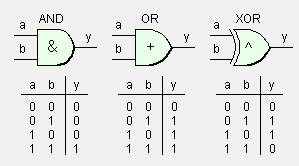
\includegraphics[width=0.3\linewidth]{images/bramki}
	\end{center}
	

	\section{Wątki a procesy - na podstawie wybranego systemu. Wymienić wady, zalety.}
	Odpowiedź

	\section{Budowa typowego układu FPGA.}
	Cechą charakterystyczną architektury FPGA jest duża liczba regularnie rozmieszczonych (w formie matrycy) konfigurowalnych komórek logicznych opartych na tablicach LUT (Look up Table), określanych generatorami funkcji. Układ FPGA zbudowany jest z programowalnych bloków logicznych oraz programowalnej macierzy połączeń. Bloki mogą być skomplikowanymi układami lub pojedynczymi bramkami logicznymi. Bloki zawierają również elementy pamięciowe (np. przerzutniki).

	\section{Podstawowe tryby adresowania systemów mikroprocesorowych}
	Odpowiedź

	\section{Hierarchia pamięci w systemie komputerowym, stronicowanie oraz koncepcja pamięci wirtualnej.}
	\begin{itemize}
		\item Rejestry wewnętrzne procesora
		\item Pamięć podręczna „cache”
		\item Pamięć operacyjna
		\item Pamięć wirtualna (dyski twarde)
	\end{itemize}

	\textbf{Stronicowanie} to metoda implementacji pamięci wirtualnej. Pamięć fizyczna dzielona jest na bloki (strony) o równych wielkościach. Adresy logiczne następnie mapowane są na odpowiednie strony oraz fizyczne adresy.
	
	\textbf{Pamięć wirtualna} pozwala na traktowanie pamięci komputera w jednolity sposób. Jeżeli program wymaga większej pamięci niż tej dostępnej, system operacyjny może wykorzystać pamięć dyskową, jednak postępowanie pozostaje bez zmian.

	\section{Omówić strukturę i funkcjonowanie systemu transmisyjnego.}
	Odpowiedź

	\section{Różnice między pamięcią statyczną i dynamiczną.}
	\begin{itemize}
		\item \textbf{SRAM} - bez zegara, bez konieczności odświeżania, niskie zużycie mocy, każda komórka składa się z 6 tranzystorów -- pamięć szybka, wysoka cena, wykorzystywana w małych ilościach (cache procesora). 
		\item \textbf{DRAM} -  wymagane cykliczne odświeżanie, każda komórka składa się z 1 tranzystora -- pamięć wolniejsza, niska cena (pamięć RAM).
	\end{itemize}

	\section{Problem synchronizacji przy transmisji danych i transmisja asynchroniczna}
	Synchroniczna i asynchroniczna metoda transmisji danych określają w jaki sposób dwie przeciwległe stacje, rozwiązują kwestię sygnalizacji nadawania danych. Bez takiej sygnalizacji, stacja odbiorcza nie byłaby w stanie odgadnąć, czy dane które akurat dotarły, to początek, koniec, czy środek transmisji.

	W transmisji asynchronicznej problem sygnalizacji początku i końca nadawania został rozwiązany dzięki temu, że została zawarta w przesyłanych danych. Czyli, to sama struktura porcji danych określa jej początek i koniec.
	W transmisji synchronicznej sygnalizacja początku i końca została rozwiązana za pomocą odrębnego kanału sygnalizującego/serwisowego. Kanał ten dyktuje takt, według którego są przesyłane dane. Natomiast dane są zwykle przesyłane odrębnymi kanałami.

	\section{Uprawnienia plików na przykładzie systemu operacyjnego Unix/Linux.}
	Nadawaniepraw odbywa się poprzez komendę \textit{chmod}. Uprawnienia plików dotyczą trzech grup:
	\begin{itemize}
		\item właściciela pliku,
		\item grupy, do której należy właściciel,
		\item pozostałych, niespełniających poprzednich warunków.
	\end{itemize}
	
	Uprawnienia dotyczą:
	\begin{itemize}
		\item odczytu,
		\item zapisu,
		\item wykonania plików
	\end{itemize}

	\section{Scharakteryzować sieciowe systemy plików.}
	p. \ref{sec:siecsysplik}

	\section{Co to jest cykl życia oprogramowania i z jakich faz się składa?}
	Ciąg działań projektowo-programowych, obejmujący zakres od powstania zapotrzebowania na oprogramowanie aż do jego wycofania z eksploatacji. Podstawowe czynności związane z tworzeniem oprogramowania:
	\begin{itemize}
		\item Określanie wymagań i specyfikacji
		\item Projektowanie
		\item Implementacja
		\item Testowanie – walidacja (atestowanie) i weryfikacja
		\item Konserwacja (pielęgnacja)
	\end{itemize}

	\section{Wymienić rodzaje diagramów w UML}
	\begin{itemize}
		\item diagram klas - przedstawia strukturę aplikacji
		\item diagram przypadków użycia - przedstawia funkcjonalność systemu wraz z jego otoczeniem, służy do zobrazowania usług, które są widoczne z zewnątrz systemu
		\item diagram sekwencji - prezentowanie interakcji pomiędzy obiektami wraz z uwzględnieniem w czasie komunikatów
		\item diagram aktywności - przedstawienie sekwencji kroków, które są wykonywane przez modelowany fragment systemu
		\item diagram komponentów - służy do ilustracji organizacji i zależności pomiędzy komponentami; prezentuje system na wyższym poziomie abstrakcji niż diagram klas, gdyż każdy z komponentów może być implementacją jednej lub większej liczby klas
	\end{itemize}

	\section{Co oznaczają skróty ERD oraz DFD? Do czego się ich używa?}
	Odpowiedź

	\section{Przeciążanie funkcji i operatorów w języku C++.}
	\label{sec:przecfuncpp}
	Przeciążanie funkcji polega na definicji funkcji o takiej samej nazwie co już istniejąca, o innych parametrach wejściowych lub wyjściowych (ale nie wyłącznie wyjściem). Przy wywołaniu funkcji, wybierana jest ta, o odpowiedniej liczbie i typach argumentów.
	Przeciążanie operatorów polega na określeniu funkcji o specjalnej nazwie operator @ dla pewnego operatora @ i typu lub typów. Niektórych operatorów nie można przeciążać, należą do nich m.in. operator ':?' oraz '.'.

	\section{Scharakteryzować instrukcje iteracyjne w przykładowym języku programowania}
	Odpowiedź

	\section{Omówić na czym polega przeciążanie funkcji i operatorów w języku C++.}
	p. \ref{sec:przecfuncpp}

	\section{Scharakteryzować mechanizmy dostępu do składowych klasy tworzonych statycznie i dynamicznie}
	Odpowiedź

	\section{Omów pojęcia agregacji i zawierania w diagramach UML.}
	Odpowiedź

	\section{Budowa i zasady działania wybranego urządzenia (drukarka laserowa, dysk twardy, pamięć USB, streamer, ect.)}
	Odpowiedź

	\section{Metody komunikacji człowiek-komputer.}
	Odpowiedź

	\section{Wymienić metody ekstrakcji wiedzy z danych.}
	Odpowiedź

	\section{Co to są drzewa decyzyjne i do czego służą?}
	Jest to graficzna metoda wspomagania procesu decyzyjnego zawierającego decyzje i ich możliwe konsekwencje. Proces decyzyjny jest przedstawiony za pomocą grafu (drzewa), gdzie wierzchołki określają aktualny stan a krawędzie pewne decyzje.

	\section{Rekurencja i jej implementacja w językach wysokiego poziomu}
	Odpowiedź

	\section{Co to są algorytmy zachłanne – podać przykład takiego algorytmu.}
	Algorytmy podejmujące w każdym kroku taką decyzję, która w danej chwili wydaje się najkorzystniejsza. Dokonują zawsze wyborów lokalnie optymalnych licząc, że doprowadzi to do znalezienia rozwiązania globalnie optymalnego. Przykład: ciągły problem plecakowy (znajduje rozwiązanie optymalne), dyskretny problem plecakowy (nie gwarantuje optymalnego rozwiązania).

	\section{Na czym polega haszowanie i gdzie ma ono zastosowanie?}
	Odpowiedź

	\section{Co to są problemy obliczeniowo trudne – podać przykład takiego problemu.}
	Problemami klasy NP nazywamy problemy decyzyjne w których sprawdzenie poprawności określonego rozwiązania wymaga złożoności obliczeniowej wielomianowej. Z powyższego stwierdzenia wynika więc, że znalezienie rozwiązania dla problemów NP wymaga złożoności co najmniej wielomianowej. Np. problem komiwojażera, plecakowy.

	\section{Maszynowa reprezentacja danych}
	Odpowiedź

	\section{Assembler, interpreter, kompilator – porównać i wyjaśnić pojęcia.}
	\begin{itemize}	
		\item \textbf{assembler}: program zamieniający kod w języku assembly na kod maszynowy,
		\item \textbf{interpreter}: program interpretujący kod pewnego języka programowania w trakcie jego wykonywania,
		\item \textbf{kompilator}: program zamieniający kod pewnego języka programowania na postać pośrednią (np. bytecode) lub kod maszynowy przed jego wykonaniem.
\end{itemize}	

	\section{Zarządzanie pamięcią w Unix/Linux.}
	Odpowiedź

	\section{Zasady korzystanie z kluczy i pakietów kryptograficznych PGP (Pretty Good Privacy)}
	Odpowiedź

	\section{Metody reprezentacji wiedzy i wnioskowanie.}
	Odpowiedź

	\section{Zasady przetwarzanie transakcji w DBMS.}
	ACID:
	\begin{itemize}
		\item \textbf{Atomicity}: atomowość, transakcja odbywa się w całości albo w ogóle,
		\item \textbf{Consistency}: spójność, transakcje nie naruszają integralności danych,
		\item \textbf{Isolation}: transakcje odbywają się bez wiedzy o innych,
		\item \textbf{Durability}: trwałość, wyniki zatwierdzonych transakcji nie mogą zostać utracone.
	\end{itemize}

	\section{Narzędzia i środowiska wytwarzania oprogramowania.}
	Odpowiedź

	\section{Wzorce projektowe i programowe.}
	Określają pewne schematy postępowania przy projektowaniu systemów bazowanych na obiektach. Podział na wzorce
	\begin{itemize}
		\item kreacyjne
			\item opisujące proces tworzenia nowych obiektów; ich zadaniem jest tworzenie, inicjalizacja oraz konfiguracja obiektów, klas oraz innych typów danych
			\item np. budowniczy, fabryka abstrakcyjna, prototyp, singleton
		\item strukturalne
		\begin{itemize}
			\item opisujące struktury powiązanych ze sobą obiektów
			\item np. adapter, dekorator, most
		\end{itemize}
		\item czynnościowe
		\begin{itemize}
			\item opisujące zachowanie i odpowiedzialność współpracujących ze sobą obiektów
			\item np. iterator, obserwator, strategia
		\end{itemize}
	\end{itemize}

	\section{Metody podnoszenia niezawodności systemów wbudowanych.}
	Odpowiedź

	\section{Ryzyko i odpowiedzialność związana z systemami informatycznymi}
	Odpowiedź

	\section{Klasyfikacja systemów oprogramowania użytkowego.}
	Odpowiedź

	\section{Systemy wspomagające wytwarzanie oprogramowania – klasyfikacja, przykłady, funkcje.}
	Odpowiedź

	\section{Wymienić i scharakteryzować podstawowe techniki w grafice komputerowej.}
	Odpowiedź

	\section{Wymienić i scharakteryzować metody przetwarzania obrazów.}
	Odpowiedź

	\section{Zasady i metody tworzenia indeksów w bazach danych?}
	Odpowiedź

	\section{Rodzaje i sposób działania przerzutników.}
	Odpowiedź

	\section{Różnica pomiędzy automatem Mealy'ego a automatem Moore'a.}
	Odpowiedź

	\section{Różnica pomiędzy układami typu PLA a układami PAL.}
	Odpowiedź

	\section{Wymienić i omówić znanych światowych wynalazców w dziedzinie informatyki i telekomunikacji}
	Odpowiedź

	\section{Omówić sposoby prezentacji informacji oraz pojęcia informacji analogowej i cyfrowej, sygnału analogowego oraz cyfrowego.}
	\textbf{Informacja}:
	\begin{itemize}
		\item Analogowa - informacje w tej postaci mogą być:
		\begin{itemize}
			\item Prosta - mocno wyróżniona jedna częstotliwość i niewielki zestaw harmonicznych (np. dźwięk jednego klawisza pianina)
			\item Złożona - składają się z wielu częstotliwości o różnym natężeniu (np. głos ludzki).
		\end{itemize}
		\item Cyfrowa - informacja z postaci impulsów elektrycznych (wartości binarnych), dyskretna.
	\end{itemize}
	\textbf{Sygnał}:
	\begin{itemize}
		\item Analogowy - jest ciągły w czasie. Jest to sinusoidalna fala o określonej częstotliwości amplitudzie i fazie. Musi być dodatkowo wzmacniany przy przesyle na większą odległość.
		\item Cyfrowy - zapisany jako zakodowane skwantyzowane wartości w pewnych odstępach czasu. Transmisje sygnału cyfrowego cechują się większym stopniem niezawodności niż analogowe zwłaszcza na dłuższych dystansach. Jeżeli nastąpi potrzeba wzmocnienia, sygnał jest regenerowany cyfrowo, co nie zwiększa mocy szumu ani zniekształceń.
	\end{itemize}


	\section{Zdefiniować pojęcie widma sygnału oraz omówić numeryczne metody jego obliczania.}
	Odpowiedź

	\section{Omówić skalę decybelewą.}
	Odpowiedź

	\section{Co to jest szerokości pasma oraz przepływności kanału transmisyjnego.}
	Odpowiedź

	\section{Omówić zagadnienie modulacji, ze szczególnym uwzględnieniem modulacji cyfrowych}
	Odpowiedź

	\section{Wymienić znane media transmisyjne.}
	Odpowiedź

	\section{Omówić problem uwierzytelniania na przykładach: uwierzytelniania SYK, uwierzytelniania SYH, uwierzytelniania SYA oraz pojęcia hasła, karty magnetycznej, karta elektronicznej, karty identyfikacyjnej SIM oraz omówić techniki biometryczne.}
	Odpowiedź

	\section{Formaty danych liczbowych.}
	Odpowiedź

	\section{Omówić zasady wykonania operacji arytmetycznych w kodzie U2.}
	Odpowiedź

	\section{Omówić zasady wykonania operacji na liczbach zmiennopozycyjnych.}
	Odpowiedź

	\section{Różnice między pamięcią statyczną i dynamiczną.}
	Odpowiedź

	\section{Wymienić standardowe postacie wyrażeń boolowskich.}
	Odpowiedź

	\section{Omówić kombinacyjne i sekwencyjne układy logiczne.}
	Kombinacyjne układy logiczne - rodzaj układów cyfrowych charakteryzujący się tym, że stan wyjść zależy wyłącznie od stanu wejść.

	Sekwencyjne układy logiczne - rodzaj układów cyfrowych charakteryzujący się tym, że stan wyjść zależy od stanu wejść układu oraz od poprzedniego stanu, zwanego stanem wewnętrznym, pamiętanego w zespole rejestrów (pamięci).

	\section{Scharakteryzować poszczególne etapy procesu konwersji analogowo-cyfrowej.}
	Odpowiedź

	\section{Omówić ogólną charakterystykę filtrów w cyfrowych.}
	Filtr cyfrowy to system, który przeprowadza operacje na spróbkowanym sygnale prowadzące do redukcji lub uwydatnienia pewnych elementów tego sygnału. Filtrowanie może przebiegać w dziedzinie czasu lub częstotliwości. W dziedzinie częstotliwości właściwości filtru opisuje transmitancja.

	Algorytm realizowany przez program komputerowy lub cyfrowy układ sekwencyjny, który w reakcji na ciąg próbek sygnału dyskretnego podanego na wejście odpowiada ciągiem próbek wyjściowych, zgodnie z deterministyczną funkcją przejścia, która może być liniowa lub nieliniowa.


	\section{Opisać proces akwizycji i kodowania danych multimedialnych w kontekście zastosowania ich w systemach transmisji strumieniowej.}
	Odpowiedź

	\section{Wymienić i omówić podstawowe parametry stosowane przy definiowaniu jakości usług.}
	Odpowiedź

	\section{Wymienić i omówić podstawowe metody szeregowania pakietów.}
	Odpowiedź

	\section{Różnica między standardami JPEG i JPEG2000, rodzaje transformacji obrazu wykorzystywane w kodowaniu obrazów.}
	Odpowiedź

	\section{Scharakteryzować kod Graya jako przykład elementu wchodzącego w skład metod cyfrowej modulacji sygnału.}
	Kod Graya charakteryzuje się tym, że dwa kolejne słowa kodowe różnią się jednym bitem. Stosowane są w korekcji błędów. Np. w modulacji cyfrowej QAM, gdzie dane są transmitowane w 4-bitowych symbolach, diagram konstelacji sygnału jest tak stworzony, aby kombinacje bitów w przylegających symbolach na konstelacji różniły się tylko jednym bitem. Po połączeniu tego z , która może korygować jednobitowe błędy, odbiornik może korygować błędy , które sprawiają, że punkty konstelacji odchylają się w stronę przyległych punktów. Dzięki temu system transmisji jest mniej podatny na zakłócenia.

	\section{Różnica między kodami detekcyjnymi i korekcyjnymi - przykłady zastosowań.}
	Odpowiedź

\end{document}